%%% Class Diagram subsection
%%% Version 2
% Class diagrams are the most common diagram type in object-oriented modeling. 
% They illustrate the static structure of a system by depicting classes, their 
% attributes, operations, and the relationships between classes. Classes 
% represent sets of objects, where attributes describe the values these objects 
% may contain, and operations specify the behaviors objects can perform.
% Associations in class diagrams describe connections between different classes, 
% with multiplicity indicators showing how many objects of one class can be linked 
% to objects of another class. Class diagrams also include other relationship types: 
% aggregation and composition (both representing whole-part relationships, with 
% different levels of dependency), and generalization (inheritance relationship 
% where specialized classes inherit properties from a general class).

% % Example here
% \begin{figure}
%     \begin{center}
%         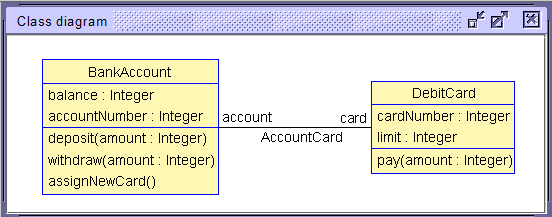
\includegraphics[width=0.8\textwidth]{figures/c1/BankAccount/BankAccount_ClassDiagram.png}
%         \caption{Class diagram of the Bank Account Model.}
%         \label{fig:class_diagram_bank_account_model}
%     \end{center}
% \end{figure}

% Figure \ref{fig:class_diagram_bank_account_model} shows an example class diagram
% of a bank account system. The system can have multiple bank accounts and each account 
% can have multiple debit cards. The class diagram consists of the classes BankAccount 
% and DebitCard with the association AccountCard. The class BankAccount has two attributes:
% - accountNumber: a unique identifier for the bank account.
% - balance: the current balance of the bank account.
% and the class DebitCard has two attributes:
% - cardNumber: a unique identifier for the debit card.
% - limit: the maximum amount that can be withdrawn using the debit card.

% The class diagram can also have other elements such as aggregation, composition
%  and generalization to show the relationship between classes. Aggregation and compo
% sition are a whole-part relationship. In aggregation, the relationship between a child
%  class and parent class is independent, whereas, in composition, they are dependent.
%  A generalization is a relationship between classes in which one class is identified as
%  the general class and the others as the specialization of it. A specialized class inherits
%  all the properties and characteristics from the general class.

%%% Version 1
% Class diagrams show the static structure of a system by depicting classes, 
% their attributes, operations, and relationships between classes. These diagrams 
% form the foundation of object-oriented modeling and capture how objects relate 
% to one another. Class diagrams are important for understanding the system structure 
% that our temporal and event-based extensions will work with.

%%% Sample
% Class diagrams are the most common diagram found in object-oriented modeling
%  systems. It illustrates the static design view of the system model and shows classes
%  of the system, their attributes, operations and associations [64]. The classes reflect
%  a set of objects. The attributes describe values that the objects may contain, and
%  an operation specifies the result of the behavior of objects. The associations describe
%  connections among the different class objects, and they can refer to each other through
%  role names. The number of objects of one class linked to other class objects depends
%  on the multiplicity attached to an association end.
% The class diagram can also have other elements such as aggregation, composition
% and generalization to show the relationship between classes. Aggregation and compo
% sition are a whole-part relationship. In aggregation, the relationship between a child
% class and parent class is independent, whereas, in composition, they are dependent.
% A generalization is a relationship between classes in which one class is identified as
% the general class and the others as the specialization of it. A specialized class inherits
% all the properties and characteristics from the general class.

%%% Object Diagram subsection
%%% Version 1
% Object diagrams provide snapshots of a system at specific points in time, showing 
% actual instances of classes (objects) and their relationships. While class diagrams 
% show abstract structures, object diagrams show concrete system states with specific 
% values. These diagrams are useful for verification purposes as they show examples 
% of system configurations that meet or violate constraints. In this thesis, object 
% diagrams play an important role in validating temporal properties through the 
% filmstrip approach.

%%% Sample
% Object diagrams are also a type of structural diagram. It represents the entitites of the
%  real world, or of the modeled system, as instances of the classes described in the class
%  diagram, and their relationships as links, which are instances of the corresponding
%  associations. Objects are defined by concrete attribute values and a link connects
%  the objects participating in the association. In general, an object diagram provides
%  a snapshot of a system at a particular point in time showing objects, their attribute
%  values, and links connecting the objects [77].
% The object diagram represents only the single state of a class diagram. So, the
%  previous state information can be lost due to the change in the system state through
%  the operation call. Therefore, a single object diagram cannot represent any flow of
%  information of a state.

%%% Sample
% The Unified Modeling Language (UML) is a graphical language for 
% visualizing, specifying, constructing, and documenting software-intensive systems.
% This unified language is maintained by the Object Management Group (OMG) [58].
% The UML has become one of the most widely used modeling language that can
% be used with all significant object and component methods for describing real-world
% application domains. Software systems, in today’s world, are growing in size, complex
% ity, distribution and importance. As a result, building and maintenance of software
% have become a more complex and challenging task. Therefore, the deployment of
% languages such as UML reduces the complexity and difficulty by providing a high
% level of abstraction, which describes precise and essential information for designing
% and developing the software system [50].  
% The graphical representation of the UML includes a set of diagrams, each focusing
% on different aspects of a design. The UML Notation Guide states all the notation of 
% diagram elements [58]. These diagrams can be classified into two groups (a) a structural
% diagram that represents the static aspect of the system, and (b) a behavioral diagram
% that describes the dynamic aspect of the system. Altogether, fourteen different model
% types can be found in the Unified Modeling Language Reference Manual [71]. In this
% thesis, two diagrams, i.e., class diagram and object diagram, have
% been extensively used and are explained further in this section.

%%% Version 3
% Class diagrams are the foundation of structural modeling in UML and the most widely used diagram type in object-oriented systems. They illustrate the static structure of a system by depicting classes, their attributes, operations, and the relationships between classes. These concepts can be observed in Figure \ref{fig:class_diagram_bank_account_model}, which shows a class diagram of a simple bank account system.

% \begin{figure}
%     \begin{center}
%         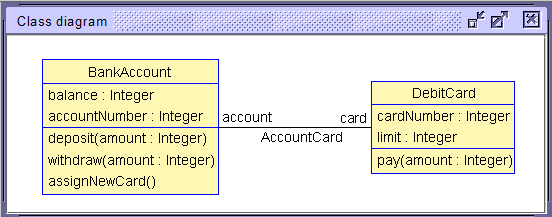
\includegraphics[width=0.8\textwidth]{figures/c1/BankAccount/BankAccount_ClassDiagram.png}
%         \caption{Class diagram of the Bank Account Model.}
%         \label{fig:class_diagram_bank_account_model}
%     \end{center}
% \end{figure}

% In this diagram, we see two classes, BankAccount and DebitCard, which represent sets of objects that share common characteristics. Each class contains attributes that describe the data values their objects may contain. The BankAccount class has attributes such as:
% \begin{itemize}
%     \item accountNumber: a unique identifier for the bank account
%     \item balance: the current balance of the bank account
% \end{itemize}

% Similarly, the DebitCard class has attributes:
% \begin{itemize}
%     \item cardNumber: a unique identifier for the debit card
%     \item limit: the maximum amount that can be withdrawn using the debit card
% \end{itemize}

% Classes also include operations that specify the behaviors objects can perform. In our example, the BankAccount class defines three operations:
% \begin{itemize}
%     \item deposit(amount): adds the specified amount to the account balance
%     \item withdraw(amount): deducts the specified amount from the balance
%     \item assignNewCard(): creates and assigns a new debit card to the bank account
% \end{itemize}
% These operations represent the functional capabilities of BankAccount objects, defining how they can interact with other objects and how their state can change over time. While attributes describe what an object knows, operations describe what an object can do.
% The relationship between these classes is represented by the AccountCard association, which connects BankAccount and DebitCard. Multiplicity indicators on this association would show how many objects of one class can be linked to objects of another class. In addition to simple associations like this one, class diagrams can include more specialized relationship types: aggregation and composition (both representing whole-part relationships with different levels of dependency), and generalization (inheritance relationships where specialized classes inherit properties from a general class).
% Class diagrams represent the static structure of a system at a particular point in time, providing the vocabulary and structural framework that other diagrams and behavioral specifications build upon.

%%% Version 2
% Object diagrams are structural diagrams that represent real-world entities or 
% modeled system elements as concrete instances of classes. While class diagrams 
% show abstract structures, object diagrams provide snapshots of a system at specific 
% points in time, showing actual objects with specific attribute values and the links 
% connecting them [77].

% Objects in these diagrams are instances of classes defined in the class diagram, 
% with concrete values assigned to their attributes. Links between objects are 
% instances of the associations defined in the class diagram. This concrete 
% representation makes object diagrams particularly valuable for verification purposes.

% % Example here
% \begin{figure}
%     \begin{center}
%         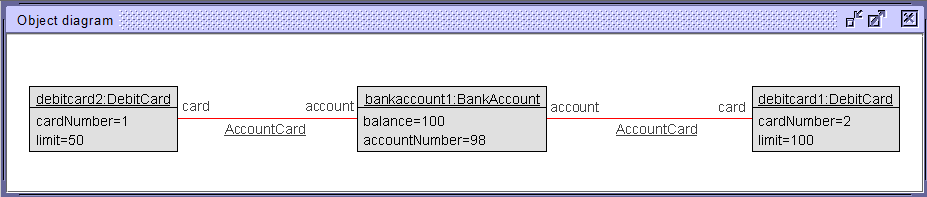
\includegraphics[width=0.8\textwidth]{figures/c1/BankAccount/BA_ObjectDiagram.png}
%         \caption{Object diagram of the Bank Account Model.}
%         \label{fig:object_diagram_bank_account_model}
%     \end{center}
% \end{figure}

% Figure \ref{fig:object_diagram_bank_account_model} shows the example object diagram, where debitcard1 and debitcard2 
% objects are instances of the class DebitCard, and bankaccount1 object is the instance of the
%  class BankAccount from the class diagram shown in Fig. \ref{fig:class_diagram_bank_account_model}. 
%  Between debitcard1, debitcard2 and bankaccount1, there exists the link AccountCard. 

% An important limitation of object diagrams is that they represent only a single 
% state of the system. When the system state changes through operation calls, 
% previous state information is lost. A single object diagram cannot represent 
% the flow of information or system evolution over time. This limitation is 
% particularly relevant to our work, as it highlights why standard UML/OCL approaches 
% struggle with temporal specifications. In this thesis, object diagrams play a crucial 
% role in our validation approach, where sequences of object diagrams (filmstrips) 
% are used to represent and verify temporal properties.

% These diagrams form the foundation of object-oriented modeling and are essential 
% for understanding the system structure that our temporal and event-based extensions 
% will work with. In this thesis, class diagrams provide the structural framework 
% upon which temporal properties will be defined and verified.
